\documentclass[conference]{IEEEtran}
\IEEEoverridecommandlockouts
% The preceding line is only needed to identify funding in the first footnote. If that is unneeded, please comment it out.
% Paquetes comunes
\usepackage[utf8]{inputenc}
\usepackage[spanish,es-tabla]{babel}  % es-tabla: "Tabla" en lugar de "Cuadro"
\usepackage{cite}
\usepackage{amsmath,amssymb,amsfonts}
\usepackage{algorithm}
\usepackage{algorithmic}
\usepackage{graphicx}
\usepackage{booktabs}
\usepackage{dblfloatfix}
\usepackage{caption}
\usepackage{subcaption}
\usepackage{rotating}
\usepackage{listings}
\usepackage{xcolor}
\usepackage{tikz}
\usetikzlibrary{arrows.meta,calc,positioning,babel}  % babel: evita el choque de < y > con babel en español
%\usepackage{pgfplots}
\usepackage{comment}

% Opciones PDF más limpias
%\pdfobjcompresslevel=0
%\pdfminorversion=4

% Enlaces e hipervínculos
\usepackage[hidelinks]{hyperref}
\usepackage{orcidlink}

\def\BibTeX{{\rm B\kern-.05em{\sc i\kern-.025em b}\kern-.08em
    T\kern-.1667em\lower.7ex\hbox{E}\kern-.125emX}}

% Ajusta una tabla al ancho de columna solo si lo excede (nunca la agranda)
\newcommand{\fitcol}[1]{\resizebox{\ifdim\width>\columnwidth\columnwidth\else\width\fi}{!}{#1}}
\begin{document}

\title{MambaLite3D: segmentación de GTVp y GTVn en PET/CT de cabeza y cuello mediante una U-Net 3D bimodal con Mamba en niveles profundos}

\author{
    \IEEEauthorblockN{ Daniel Frank Quiñones-Olgado}
        \IEEEauthorblockA{
        \textit{Universidad Nacional de San Agustín de Arequipa}\\ Arequipa, Perú \\
        \href{mailto:dquinoneso@unsa.edu.pe}{dquinoneso@unsa.edu.pe}}
    \and

    \IEEEauthorblockN{ Percy Maldonado-Quispe}
        \IEEEauthorblockA{
        \textit{Universidad Nacional de San Agustín de Arequipa}\\ Arequipa, Perú \\
        \href{mailto:pmaldonado@unsa.edu.pe}{pmaldonado@unsa.edu.pe}
        \orcidlink{0009-0007-6391-5370}}
}

\maketitle
\begin{abstract}
La segmentación automática del tumor primario (GTVp) y de los ganglios linfáticos metastásicos (GTVn) en PET/CT de cabeza y cuello es necesaria para la planificación del tratamiento, pero sigue siendo difícil por la variabilidad entre centros, las estructuras pequeñas y los bordes poco definidos. Presentamos MambaLite3D, una U-Net 3D bimodal (PET y CT) que incorpora bloques Mamba solo en los niveles más profundos (los dos últimos del codificador y del decodificador, y el cuello de botella), junto con módulos de mezcla multidireccional (AMF3D), de atención local-global (LGFM3D) y de atención cruzada en las conexiones skip (CGA3D). El modelo, de 15.8 M de parámetros, se entrenó sobre 476 casos de HECKTOR 2025 con un protocolo estratificado por centro (70/20/10) y se evaluó con las métricas oficiales de HECKTOR 2025 y 2022. En el conjunto de test (69 casos), con postprocesado ajustado solo en validación, obtuvo un DSC de GTVp de 0.711, un DSC agregado de GTVn de 0.740 y un F1 de detección de GTVn de 0.703. Frente a la variante base de la misma arquitectura (4.0 M de parámetros), evaluada con el mismo protocolo, las diferencias en test son pequeñas y no se han sometido todavía a una prueba estadística pareada.
\end{abstract}

\renewcommand{\IEEEkeywordsname}{Palabras clave}
\begin{IEEEkeywords}
Segmentación médica, PET/CT, cáncer de cabeza y cuello, HECKTOR 2025, Mamba, modelos de espacio de estados, U-Net 3D
\end{IEEEkeywords}

\section{Introducción}
El cáncer de cabeza y cuello es uno de los tipos de cáncer más frecuentes a nivel mundial \cite{Li_2023}. % VERIFICAR: la fuente original de la cifra de incidencia (4 % en EE. UU.) no está confirmada; se retiró el porcentaje.
En su manejo clínico, la delimitación del tumor primario (GTVp) y de los ganglios linfáticos metastásicos (GTVn) en imágenes de tomografía por emisión de positrones (PET) y de tomografía computarizada (CT) es un paso central del diagnóstico, de la planificación de la radioterapia y del seguimiento \cite{isa_net2023}. Ambas modalidades son complementarias: la CT aporta el detalle anatómico y la PET refleja la actividad metabólica del tejido tumoral \cite{SegmentationHeadNeckDualPETCT2025}.

La delimitación manual es lenta y presenta variabilidad entre especialistas. En cabeza y cuello, a ello se suman la complejidad anatómica, el tamaño reducido de muchas lesiones, los bordes poco definidos y la gran variabilidad de forma e intensidad entre pacientes \cite{Chu2023114}. Estas limitaciones han motivado el desarrollo de métodos automáticos de segmentación, evaluados en desafíos multicéntricos como HECKTOR \cite{Oreiller2022,saeed2026hecktor25}.

Las redes convolucionales (CNN) modelan bien la información local, pero su campo receptivo limitado dificulta capturar dependencias espaciales de largo alcance. Los Transformers abordan esta limitación mediante autoatención \cite{vaswani2023attentionneed,dosovitskiy2021imageworth16x16words}, con un coste cuadrático en la longitud de la secuencia y una alta demanda de datos y de memoria \cite{ANDRADEMIRANDA2023102308}. Los modelos de espacio de estados (SSM), y en particular Mamba \cite{gu2023mamba}, capturan dependencias de largo alcance con coste lineal y ya se han incorporado a la segmentación médica 3D \cite{ma2024umamba,xing2024segmamba}. Hasta donde revisamos, su aplicación a PET/CT bimodal de cabeza y cuello con el protocolo de HECKTOR 2025 no se ha explorado, y las comparaciones entre trabajos suelen mezclar particiones y métricas distintas.

En este trabajo proponemos MambaLite3D, una U-Net 3D bimodal que incorpora bloques Mamba únicamente en los niveles más profundos, donde la secuencia de tokens es corta y el coste computacional es bajo. El diseño, adaptado de MambaLiteUNet y SegMamba, combina estos bloques con una mezcla multidireccional con cuatro órdenes de barrido (AMF3D), una atención global-local (LGFM3D) y una atención cruzada en las conexiones de salto (CGA3D). Lo evaluamos con un protocolo reproducible sobre HECKTOR 2025, con una partición estratificada por centro (70/20/10), preprocesamiento y ROI calculados al vuelo y las métricas de HECKTOR 2025 y 2022. Bajo ese mismo protocolo comparamos dos tamaños de la arquitectura, de 4.0 M y 15.8 M de parámetros, con un postprocesado a nivel de componentes conexas ajustado únicamente en validación. Además, reportamos el consumo de memoria de GPU y los tiempos de entrenamiento e inferencia en una GPU de 4 GB, un aspecto determinante para su uso en equipos con recursos limitados.

El resto del artículo se organiza así: la Sección~\ref{sec:state} revisa los trabajos relacionados, la Sección~\ref{sec:arquitectura} describe el método, la Sección~\ref{sec:results} presenta los resultados, la Sección~\ref{sec:discusion} los discute y la Sección~\ref{sec:conclusiones} concluye.

\section{Trabajos Relacionados}
\label{sec:state}

Las CNN son la base de la segmentación médica 3D, porque extraen características jerárquicas y combinan información local y global mediante convolución, reducción y reconstrucción de resolución. nnU-Net \cite{isensee2021nnunet} fijó un estándar de referencia al configurar automáticamente la arquitectura y el entrenamiento a partir de los datos. En PET/CT de cabeza y cuello, Ren et al. \cite{REN2021} emplearon nnU-Net 3D con normalizaciones específicas de PET y alcanzaron un DSC de 0.779 y un HD95 de 3.15 mm en HECKTOR 2021; Douglas et al. \cite{DOUGLAS2025110309} combinaron una V-Net 3D con optimización bayesiana en dos fases y obtuvieron un DSC medio de 0.764 en validación cruzada de diez pliegues; y Huang et al. \cite{isa_net2023} conectaron dos U-Net 3D mediante atención espacial y de canal (ISA-Net), con un DSC de 0.8076 en HECKTOR 2021 y de 0.8378 en el conjunto STS.

La limitada capacidad de las CNN para modelar dependencias de largo alcance motivó los modelos híbridos CNN–Transformer, que combinan convoluciones locales con atención global. Mohammed et al. \cite{SegmentationHeadNeckDualPETCT2025} compararon variantes 2D, 2.5D y 3D de una UNet Transformer y encontraron en la 2.5D el mejor equilibrio entre precisión y coste, con un Dice de 0.818 en HECKTOR 2022. Chu et al. \cite{Chu2023114} aplicaron Swin UNETR con transferencia de aprendizaje y obtuvieron un Dice medio de 0.656 en el conjunto de prueba de HECKTOR 2022. En la fusión de modalidades, Mahdi et al. \cite{MAHDI2024} propusieron una fusión ponderada entre PET y CT, con un Dice máximo de 0.649, y Li et al. \cite{Li_2023} introdujeron la atención cruzada entre modalidades de SwinCross, con un Dice medio de 0.769 en HECKTOR 2021.

El coste cuadrático de la atención ha impulsado, más recientemente, el uso de modelos de espacio de estados. Mamba \cite{gu2023mamba} sustituye la atención por un barrido selectivo con coste lineal en la longitud de la secuencia. En segmentación médica, U-Mamba \cite{ma2024umamba} incorporó bloques Mamba a una U-Net, SegMamba \cite{xing2024segmamba} los extendió a volúmenes 3D con barridos en varias direcciones y VM-UNet \cite{ruan2024vmunet} los adaptó a arquitecturas U-Net 2D. MambaLiteUNet \cite{rahman2026mambalite}, base del diseño que proponemos, reduce el coste de estos modelos. Hasta donde revisamos, no hay trabajos publicados que apliquen estos bloques a PET/CT de cabeza y cuello con el protocolo de HECKTOR 2025. En conjunto, la literatura muestra una evolución desde las CNN hacia los híbridos con Transformers y los SSM, pero las comparaciones directas son difíciles, porque cada estudio emplea su propia edición del desafío, su propia partición y su propia métrica.

% Iniciar sección de Arquitectura Propuesta
\section{Método Propuesto}
\label{sec:arquitectura}
\subsection{Dataset}

Usamos el conjunto de datos HECKTOR 2025 (Tarea 1) \cite{saeed2026hecktor25,saeed2025dataset}, una colección multicéntrica de estudios PET/CT de pacientes con cáncer de cabeza y cuello, con anotaciones manuales del tumor primario (GTVp) y de los ganglios metastásicos (GTVn). Los 680 casos proceden de siete centros, con distintos protocolos de adquisición y resoluciones.

La partición es estratificada por centro, con proporciones 70/20/10 (Tabla~\ref{tab:split}), que también muestra la distribución de casos por centro. Cada centro aporta a los tres subconjuntos, de modo que el test refleja la misma distribución de centros que el entrenamiento. La semilla es 12345.

\begin{table}[!t]
\centering
\caption{Casos por centro en HECKTOR 2025 y partición estratificada 70/20/10.}
\label{tab:split}
\footnotesize
\begin{tabular}{l r r r r}
\hline
Centro & Total & Entrenamiento & Validación & Test \\
\hline
CHUM & 56 & 39 & 11 & 6 \\
CHUP & 72 & 51 & 14 & 7 \\
CHUS & 72 & 51 & 14 & 7 \\
HGJ & 55 & 38 & 11 & 6 \\
HMR & 18 & 12 & 4 & 2 \\
MDA & 396 & 277 & 79 & 40 \\
USZ & 11 & 8 & 2 & 1 \\
\hline
Total & 680 & 476 & 135 & 69 \\
Proporción & 100 \% & 70 \% & 20 \% & 10 \% \\
\hline
\end{tabular}
\end{table}

\subsection{Preprocesamiento y ROI}

Ambas modalidades se remuestrean a una rejilla común de 1.0 × 1.0 × 3.0 mm (x, y, z). Las máscaras se remuestrean con vecino más cercano para conservar las etiquetas. En la CT, los valores se truncan al intervalo $[-200, 400]$ UH y se escalan a $[0, 1]$. En la PET, el SUV se recorta a 5 y se normaliza con z-score.

El ROI se calcula por caso para reducir el volumen procesado. Se construye una máscara de cuerpo a partir de la CT ($> -500$ UH) o de la PET ($\mathrm{SUV} > 0.5$), se aplica una apertura morfológica de dos vóxeles y se conserva la componente conexa mayor. Esta componente elimina la camilla y el reposacabezas, que de otro modo ocupan casi todo el campo de visión. El extremo superior del ROI es el corte más alto del cuerpo con $\mathrm{SUV} > 2$, y el ROI se extiende 270 mm hacia abajo. Se añade un margen de 8 vóxeles en cada dirección y un tamaño mínimo de $96 \times 96 \times 32$ vóxeles. En el conjunto de entrenamiento, la etiqueta queda al 100 \% dentro del ROI.

Los casos se leen de los NIfTI originales y se preprocesan al vuelo. No se escribe ninguna copia del conjunto de datos en disco. Una caché rodante de 60 casos (unos 3.7 GB en RAM) se renueva con 10 casos por época.

\subsection{Arquitectura del modelo}

MambaLite3D es una U-Net 3D con dos entradas (PET y CT) y tres salidas (fondo, GTVp y GTVn). Tiene seis niveles, con canales $[24, 32, 64, 96, 128, 192]$, y los strides y núcleos se derivan del tamaño del parche y del espaciado, siguiendo la heurística de nnU-Net. El tamaño de entrada es de $32 \times 128 \times 128$ vóxeles. El modelo tiene 15.8 M de parámetros. La Fig.~\ref{fig:arquitectura} resume la arquitectura.

\begin{figure*}[!t]
\centering
\resizebox{\textwidth}{!}{% Diagrama de MambaLite3D (variante wide). Requiere tikz con las librerías arrows.meta y calc.
% Se incluye en el paper con % Diagrama de MambaLite3D (variante wide). Requiere tikz con las librerías arrows.meta y calc.
% Se incluye en el paper con % Diagrama de MambaLite3D (variante wide). Requiere tikz con las librerías arrows.meta y calc.
% Se incluye en el paper con \input{figuras/arquitectura_tikz} y como PNG con arquitectura_standalone.tex.
\begin{tikzpicture}[
    font=\scriptsize,
    >={Stealth[length=4pt]},
    bloque/.style={draw=black!55, fill=black!6, rounded corners=2pt, minimum width=3.1cm,
                   minimum height=0.68cm, align=center, inner sep=2pt},
    conv/.style={bloque, fill=blue!9, draw=blue!45!black},
    mamba/.style={bloque, fill=orange!28, draw=orange!70!black},
    cga/.style={draw=teal!70!black, fill=teal!18, rounded corners=2pt, minimum width=1.25cm,
                minimum height=0.5cm, align=center},
    fue/.style={draw=black!50, fill=black!8, rounded corners=2pt, minimum width=1.25cm,
                minimum height=0.5cm, align=center},
    suma/.style={circle, draw=black!70, fill=white, inner sep=0pt, minimum size=0.36cm},
    cabeza/.style={draw=black!50, fill=white, rounded corners=2pt, minimum width=1.5cm,
                   minimum height=0.5cm, align=center},
    io/.style={draw=black!70, fill=white, rounded corners=2pt, minimum width=3.1cm,
               minimum height=0.68cm, align=center},
    flecha/.style={->, draw=black!70, line width=0.6pt},
    salto/.style={->, draw=black!60, line width=0.6pt},
    compuerta/.style={->, draw=teal!70!black, dashed, line width=0.5pt},
    etq/.style={font=\tiny, text=black!70},
]
\def\xe{0}      % columna del codificador
\def\xs{5.0}    % columna de las conexiones de salto
\def\xf{7.6}    % columna de las sumas
\def\xd{10.0}   % columna del decodificador
\def\xh{13.2}   % columna de las cabezas de supervisión
\def\dy{1.15}

% ---------------- entrada y codificador ----------------
\node[io] (in) at (\xe, 1.25) {Entrada: CT + PET\\$2\times32\times128\times128$};
\node[conv]  (e0) at (\xe, 0)          {Conv + Res\\24 \,·\, $32{\times}128{\times}128$};
\node[conv]  (e1) at (\xe, -1*\dy)     {Stem DW 7 + Res\\32 \,·\, $32{\times}64{\times}64$};
\node[conv]  (e2) at (\xe, -2*\dy)     {Conv + Res\\64 \,·\, $16{\times}32{\times}32$};
\node[conv]  (e3) at (\xe, -3*\dy)     {Conv + Res\\96 \,·\, $8{\times}16{\times}16$};
\node[mamba] (e4) at (\xe, -4*\dy)     {MambaStage\\128 \,·\, $4{\times}8{\times}8$};
\node[mamba] (e5) at (\xe, -5*\dy)     {MambaStage\\192 \,·\, $4{\times}4{\times}4$};
\node[mamba, minimum width=4.2cm] (b) at ({(\xe+\xf)/2}, -6.1*\dy)
     {Cuello de botella: MambaStage\\256 \,·\, $4{\times}4{\times}4$};

\draw[flecha] (in) -- (e0);
\draw[flecha] (e0) -- node[etq, right] {DW conv, $s{=}(1,2,2)$} (e1);
\draw[flecha] (e1) -- node[etq, right] {MaxPool $(2,2,2)$} (e2);
\draw[flecha] (e2) -- node[etq, right] {MaxPool $(2,2,2)$} (e3);
\draw[flecha] (e3) -- node[etq, right] {MaxPool $(2,2,2)$} (e4);
\draw[flecha] (e4) -- node[etq, right] {MaxPool $(1,2,2)$} (e5);
\draw[flecha] (e5.south) |- (b.west);

% ---------------- decodificador ----------------
\node[conv]  (d0) at (\xd, 0)          {Res\\24};
\node[conv]  (d1) at (\xd, -1*\dy)     {Res\\32};
\node[conv]  (d2) at (\xd, -2*\dy)     {Res\\64};
\node[conv]  (d3) at (\xd, -3*\dy)     {Res\\96};
\node[mamba] (d4) at (\xd, -4*\dy)     {MambaStage\\128};
\node[mamba] (d5) at (\xd, -5*\dy)     {MambaStage\\192};
\node[io]    (out) at (\xd, 1.25)      {Salida: 3 clases\\fondo, GTVp, GTVn};
\draw[flecha] (d0) -- node[etq, right] {Conv $1{\times}1$ + softmax ($w{=}0.53$)} (out);

% sumas, conexiones de salto y caminos de subida
\foreach \i in {0,...,5} {
    \node[suma] (f\i) at (\xf, -\i*\dy) {$+$};
    \draw[flecha] (f\i) -- (d\i);
}
\foreach \i in {0,1,2} {
    \node[fue] (s\i) at (\xs, -\i*\dy) {FUE};
}
\foreach \i in {3,4,5} {
    \node[cga] (s\i) at (\xs, -\i*\dy) {CGA3D};
}
\foreach \i in {0,...,5} {
    \draw[salto] (e\i) -- (s\i);
    \draw[salto] (s\i) -- (f\i);
}
% subida desde el nivel inferior: ConvTranspose (o conv 1x1 desde el cuello de botella).
% Sale del borde superior del bloque de abajo, sube por el hueco entre filas y entra a la suma por debajo.
\def\xu{8.95}
\foreach \i/\j in {0/1,1/2,2/3,3/4,4/5} {
    \draw[flecha] (\xu, -\j*\dy+0.34) -- (\xu, -\i*\dy-0.55) -- (\xf, -\i*\dy-0.55) -- (f\i.south);
    \node[etq, anchor=west] at (\xu+0.05, -\i*\dy-0.66) {ConvT};
}
\draw[flecha] (b.east) -| (f5.south);
\node[etq, anchor=west] at (\xf+0.05, -6.1*\dy+0.2) {Conv $1{\times}1$};
% compuerta de CGA3D: usa el mapa del decodificador que llega a la suma
\foreach \i in {3,4,5} {
    \draw[compuerta] (\xf, -\i*\dy-0.55) -| (s\i.south);
}

% supervisión profunda
\foreach \i/\w in {1/0.27,2/0.13,3/0.07,4/0} {
    \node[cabeza] (h\i) at (\xh, -\i*\dy) {Conv $1{\times}1$\\$w{=}\w$};
    \draw[flecha] (d\i) -- (h\i);
}
\node[etq, above=1pt of h1, align=center] {Supervisión\\profunda};

% ---------------- detalle de MambaStage ----------------
\begin{scope}[shift={(0,-8.35)}]
    \node[font=\scriptsize\bfseries, anchor=west] at (-1.6, 0.75) {MambaStage};
    \tikzset{paso/.style={draw=orange!70!black, fill=orange!14, rounded corners=2pt,
                          minimum height=0.62cm, align=center, inner sep=3pt}}
    \node[paso] (m0) at (-0.6, 0)  {Proy. $1{\times}1$\\+ norm.};
    \node[paso, right=0.45cm of m0] (m1) {GSC3D};
    \node[paso, right=0.45cm of m1] (m2) {AMF3D\\4 grupos: fwd, rev, slice, ap};
    \node[paso, right=0.45cm of m2] (m3) {LGFM3D\\conv DW local + atención global};
    \node[paso, right=0.45cm of m3] (m4) {LN + proy.\\$1{\times}1$};
    \draw[flecha] (m0) -- (m1);
    \draw[flecha] (m1) -- (m2);
    \draw[flecha] (m2) -- (m3);
    \draw[flecha] (m3) -- (m4);
\end{scope}

% ---------------- leyenda ----------------
\begin{scope}[shift={(0,-9.6)}]
    \tikzset{muestra/.style={minimum width=0.5cm, minimum height=0.3cm}}
    \node[conv, muestra] (l1) at (-1.3, 0) {};
    \node[anchor=west] (t1) at (l1.east) {Bloque convolucional residual};
    \node[mamba, muestra, right=0.5cm of t1] (l2) {};
    \node[anchor=west] (t2) at (l2.east) {Bloque con Mamba};
    \node[cga, muestra, right=0.5cm of t2] (l3) {};
    \node[anchor=west] (t3) at (l3.east) {Atención cruzada (CGA3D)};
    \node[fue, muestra, right=0.5cm of t3] (l4) {};
    \node[anchor=west] at (l4.east) {FUE (sin parámetros)};
\end{scope}
\end{tikzpicture}
 y como PNG con arquitectura_standalone.tex.
\begin{tikzpicture}[
    font=\scriptsize,
    >={Stealth[length=4pt]},
    bloque/.style={draw=black!55, fill=black!6, rounded corners=2pt, minimum width=3.1cm,
                   minimum height=0.68cm, align=center, inner sep=2pt},
    conv/.style={bloque, fill=blue!9, draw=blue!45!black},
    mamba/.style={bloque, fill=orange!28, draw=orange!70!black},
    cga/.style={draw=teal!70!black, fill=teal!18, rounded corners=2pt, minimum width=1.25cm,
                minimum height=0.5cm, align=center},
    fue/.style={draw=black!50, fill=black!8, rounded corners=2pt, minimum width=1.25cm,
                minimum height=0.5cm, align=center},
    suma/.style={circle, draw=black!70, fill=white, inner sep=0pt, minimum size=0.36cm},
    cabeza/.style={draw=black!50, fill=white, rounded corners=2pt, minimum width=1.5cm,
                   minimum height=0.5cm, align=center},
    io/.style={draw=black!70, fill=white, rounded corners=2pt, minimum width=3.1cm,
               minimum height=0.68cm, align=center},
    flecha/.style={->, draw=black!70, line width=0.6pt},
    salto/.style={->, draw=black!60, line width=0.6pt},
    compuerta/.style={->, draw=teal!70!black, dashed, line width=0.5pt},
    etq/.style={font=\tiny, text=black!70},
]
\def\xe{0}      % columna del codificador
\def\xs{5.0}    % columna de las conexiones de salto
\def\xf{7.6}    % columna de las sumas
\def\xd{10.0}   % columna del decodificador
\def\xh{13.2}   % columna de las cabezas de supervisión
\def\dy{1.15}

% ---------------- entrada y codificador ----------------
\node[io] (in) at (\xe, 1.25) {Entrada: CT + PET\\$2\times32\times128\times128$};
\node[conv]  (e0) at (\xe, 0)          {Conv + Res\\24 \,·\, $32{\times}128{\times}128$};
\node[conv]  (e1) at (\xe, -1*\dy)     {Stem DW 7 + Res\\32 \,·\, $32{\times}64{\times}64$};
\node[conv]  (e2) at (\xe, -2*\dy)     {Conv + Res\\64 \,·\, $16{\times}32{\times}32$};
\node[conv]  (e3) at (\xe, -3*\dy)     {Conv + Res\\96 \,·\, $8{\times}16{\times}16$};
\node[mamba] (e4) at (\xe, -4*\dy)     {MambaStage\\128 \,·\, $4{\times}8{\times}8$};
\node[mamba] (e5) at (\xe, -5*\dy)     {MambaStage\\192 \,·\, $4{\times}4{\times}4$};
\node[mamba, minimum width=4.2cm] (b) at ({(\xe+\xf)/2}, -6.1*\dy)
     {Cuello de botella: MambaStage\\256 \,·\, $4{\times}4{\times}4$};

\draw[flecha] (in) -- (e0);
\draw[flecha] (e0) -- node[etq, right] {DW conv, $s{=}(1,2,2)$} (e1);
\draw[flecha] (e1) -- node[etq, right] {MaxPool $(2,2,2)$} (e2);
\draw[flecha] (e2) -- node[etq, right] {MaxPool $(2,2,2)$} (e3);
\draw[flecha] (e3) -- node[etq, right] {MaxPool $(2,2,2)$} (e4);
\draw[flecha] (e4) -- node[etq, right] {MaxPool $(1,2,2)$} (e5);
\draw[flecha] (e5.south) |- (b.west);

% ---------------- decodificador ----------------
\node[conv]  (d0) at (\xd, 0)          {Res\\24};
\node[conv]  (d1) at (\xd, -1*\dy)     {Res\\32};
\node[conv]  (d2) at (\xd, -2*\dy)     {Res\\64};
\node[conv]  (d3) at (\xd, -3*\dy)     {Res\\96};
\node[mamba] (d4) at (\xd, -4*\dy)     {MambaStage\\128};
\node[mamba] (d5) at (\xd, -5*\dy)     {MambaStage\\192};
\node[io]    (out) at (\xd, 1.25)      {Salida: 3 clases\\fondo, GTVp, GTVn};
\draw[flecha] (d0) -- node[etq, right] {Conv $1{\times}1$ + softmax ($w{=}0.53$)} (out);

% sumas, conexiones de salto y caminos de subida
\foreach \i in {0,...,5} {
    \node[suma] (f\i) at (\xf, -\i*\dy) {$+$};
    \draw[flecha] (f\i) -- (d\i);
}
\foreach \i in {0,1,2} {
    \node[fue] (s\i) at (\xs, -\i*\dy) {FUE};
}
\foreach \i in {3,4,5} {
    \node[cga] (s\i) at (\xs, -\i*\dy) {CGA3D};
}
\foreach \i in {0,...,5} {
    \draw[salto] (e\i) -- (s\i);
    \draw[salto] (s\i) -- (f\i);
}
% subida desde el nivel inferior: ConvTranspose (o conv 1x1 desde el cuello de botella).
% Sale del borde superior del bloque de abajo, sube por el hueco entre filas y entra a la suma por debajo.
\def\xu{8.95}
\foreach \i/\j in {0/1,1/2,2/3,3/4,4/5} {
    \draw[flecha] (\xu, -\j*\dy+0.34) -- (\xu, -\i*\dy-0.55) -- (\xf, -\i*\dy-0.55) -- (f\i.south);
    \node[etq, anchor=west] at (\xu+0.05, -\i*\dy-0.66) {ConvT};
}
\draw[flecha] (b.east) -| (f5.south);
\node[etq, anchor=west] at (\xf+0.05, -6.1*\dy+0.2) {Conv $1{\times}1$};
% compuerta de CGA3D: usa el mapa del decodificador que llega a la suma
\foreach \i in {3,4,5} {
    \draw[compuerta] (\xf, -\i*\dy-0.55) -| (s\i.south);
}

% supervisión profunda
\foreach \i/\w in {1/0.27,2/0.13,3/0.07,4/0} {
    \node[cabeza] (h\i) at (\xh, -\i*\dy) {Conv $1{\times}1$\\$w{=}\w$};
    \draw[flecha] (d\i) -- (h\i);
}
\node[etq, above=1pt of h1, align=center] {Supervisión\\profunda};

% ---------------- detalle de MambaStage ----------------
\begin{scope}[shift={(0,-8.35)}]
    \node[font=\scriptsize\bfseries, anchor=west] at (-1.6, 0.75) {MambaStage};
    \tikzset{paso/.style={draw=orange!70!black, fill=orange!14, rounded corners=2pt,
                          minimum height=0.62cm, align=center, inner sep=3pt}}
    \node[paso] (m0) at (-0.6, 0)  {Proy. $1{\times}1$\\+ norm.};
    \node[paso, right=0.45cm of m0] (m1) {GSC3D};
    \node[paso, right=0.45cm of m1] (m2) {AMF3D\\4 grupos: fwd, rev, slice, ap};
    \node[paso, right=0.45cm of m2] (m3) {LGFM3D\\conv DW local + atención global};
    \node[paso, right=0.45cm of m3] (m4) {LN + proy.\\$1{\times}1$};
    \draw[flecha] (m0) -- (m1);
    \draw[flecha] (m1) -- (m2);
    \draw[flecha] (m2) -- (m3);
    \draw[flecha] (m3) -- (m4);
\end{scope}

% ---------------- leyenda ----------------
\begin{scope}[shift={(0,-9.6)}]
    \tikzset{muestra/.style={minimum width=0.5cm, minimum height=0.3cm}}
    \node[conv, muestra] (l1) at (-1.3, 0) {};
    \node[anchor=west] (t1) at (l1.east) {Bloque convolucional residual};
    \node[mamba, muestra, right=0.5cm of t1] (l2) {};
    \node[anchor=west] (t2) at (l2.east) {Bloque con Mamba};
    \node[cga, muestra, right=0.5cm of t2] (l3) {};
    \node[anchor=west] (t3) at (l3.east) {Atención cruzada (CGA3D)};
    \node[fue, muestra, right=0.5cm of t3] (l4) {};
    \node[anchor=west] at (l4.east) {FUE (sin parámetros)};
\end{scope}
\end{tikzpicture}
 y como PNG con arquitectura_standalone.tex.
\begin{tikzpicture}[
    font=\scriptsize,
    >={Stealth[length=4pt]},
    bloque/.style={draw=black!55, fill=black!6, rounded corners=2pt, minimum width=3.1cm,
                   minimum height=0.68cm, align=center, inner sep=2pt},
    conv/.style={bloque, fill=blue!9, draw=blue!45!black},
    mamba/.style={bloque, fill=orange!28, draw=orange!70!black},
    cga/.style={draw=teal!70!black, fill=teal!18, rounded corners=2pt, minimum width=1.25cm,
                minimum height=0.5cm, align=center},
    fue/.style={draw=black!50, fill=black!8, rounded corners=2pt, minimum width=1.25cm,
                minimum height=0.5cm, align=center},
    suma/.style={circle, draw=black!70, fill=white, inner sep=0pt, minimum size=0.36cm},
    cabeza/.style={draw=black!50, fill=white, rounded corners=2pt, minimum width=1.5cm,
                   minimum height=0.5cm, align=center},
    io/.style={draw=black!70, fill=white, rounded corners=2pt, minimum width=3.1cm,
               minimum height=0.68cm, align=center},
    flecha/.style={->, draw=black!70, line width=0.6pt},
    salto/.style={->, draw=black!60, line width=0.6pt},
    compuerta/.style={->, draw=teal!70!black, dashed, line width=0.5pt},
    etq/.style={font=\tiny, text=black!70},
]
\def\xe{0}      % columna del codificador
\def\xs{5.0}    % columna de las conexiones de salto
\def\xf{7.6}    % columna de las sumas
\def\xd{10.0}   % columna del decodificador
\def\xh{13.2}   % columna de las cabezas de supervisión
\def\dy{1.15}

% ---------------- entrada y codificador ----------------
\node[io] (in) at (\xe, 1.25) {Entrada: CT + PET\\$2\times32\times128\times128$};
\node[conv]  (e0) at (\xe, 0)          {Conv + Res\\24 \,·\, $32{\times}128{\times}128$};
\node[conv]  (e1) at (\xe, -1*\dy)     {Stem DW 7 + Res\\32 \,·\, $32{\times}64{\times}64$};
\node[conv]  (e2) at (\xe, -2*\dy)     {Conv + Res\\64 \,·\, $16{\times}32{\times}32$};
\node[conv]  (e3) at (\xe, -3*\dy)     {Conv + Res\\96 \,·\, $8{\times}16{\times}16$};
\node[mamba] (e4) at (\xe, -4*\dy)     {MambaStage\\128 \,·\, $4{\times}8{\times}8$};
\node[mamba] (e5) at (\xe, -5*\dy)     {MambaStage\\192 \,·\, $4{\times}4{\times}4$};
\node[mamba, minimum width=4.2cm] (b) at ({(\xe+\xf)/2}, -6.1*\dy)
     {Cuello de botella: MambaStage\\256 \,·\, $4{\times}4{\times}4$};

\draw[flecha] (in) -- (e0);
\draw[flecha] (e0) -- node[etq, right] {DW conv, $s{=}(1,2,2)$} (e1);
\draw[flecha] (e1) -- node[etq, right] {MaxPool $(2,2,2)$} (e2);
\draw[flecha] (e2) -- node[etq, right] {MaxPool $(2,2,2)$} (e3);
\draw[flecha] (e3) -- node[etq, right] {MaxPool $(2,2,2)$} (e4);
\draw[flecha] (e4) -- node[etq, right] {MaxPool $(1,2,2)$} (e5);
\draw[flecha] (e5.south) |- (b.west);

% ---------------- decodificador ----------------
\node[conv]  (d0) at (\xd, 0)          {Res\\24};
\node[conv]  (d1) at (\xd, -1*\dy)     {Res\\32};
\node[conv]  (d2) at (\xd, -2*\dy)     {Res\\64};
\node[conv]  (d3) at (\xd, -3*\dy)     {Res\\96};
\node[mamba] (d4) at (\xd, -4*\dy)     {MambaStage\\128};
\node[mamba] (d5) at (\xd, -5*\dy)     {MambaStage\\192};
\node[io]    (out) at (\xd, 1.25)      {Salida: 3 clases\\fondo, GTVp, GTVn};
\draw[flecha] (d0) -- node[etq, right] {Conv $1{\times}1$ + softmax ($w{=}0.53$)} (out);

% sumas, conexiones de salto y caminos de subida
\foreach \i in {0,...,5} {
    \node[suma] (f\i) at (\xf, -\i*\dy) {$+$};
    \draw[flecha] (f\i) -- (d\i);
}
\foreach \i in {0,1,2} {
    \node[fue] (s\i) at (\xs, -\i*\dy) {FUE};
}
\foreach \i in {3,4,5} {
    \node[cga] (s\i) at (\xs, -\i*\dy) {CGA3D};
}
\foreach \i in {0,...,5} {
    \draw[salto] (e\i) -- (s\i);
    \draw[salto] (s\i) -- (f\i);
}
% subida desde el nivel inferior: ConvTranspose (o conv 1x1 desde el cuello de botella).
% Sale del borde superior del bloque de abajo, sube por el hueco entre filas y entra a la suma por debajo.
\def\xu{8.95}
\foreach \i/\j in {0/1,1/2,2/3,3/4,4/5} {
    \draw[flecha] (\xu, -\j*\dy+0.34) -- (\xu, -\i*\dy-0.55) -- (\xf, -\i*\dy-0.55) -- (f\i.south);
    \node[etq, anchor=west] at (\xu+0.05, -\i*\dy-0.66) {ConvT};
}
\draw[flecha] (b.east) -| (f5.south);
\node[etq, anchor=west] at (\xf+0.05, -6.1*\dy+0.2) {Conv $1{\times}1$};
% compuerta de CGA3D: usa el mapa del decodificador que llega a la suma
\foreach \i in {3,4,5} {
    \draw[compuerta] (\xf, -\i*\dy-0.55) -| (s\i.south);
}

% supervisión profunda
\foreach \i/\w in {1/0.27,2/0.13,3/0.07,4/0} {
    \node[cabeza] (h\i) at (\xh, -\i*\dy) {Conv $1{\times}1$\\$w{=}\w$};
    \draw[flecha] (d\i) -- (h\i);
}
\node[etq, above=1pt of h1, align=center] {Supervisión\\profunda};

% ---------------- detalle de MambaStage ----------------
\begin{scope}[shift={(0,-8.35)}]
    \node[font=\scriptsize\bfseries, anchor=west] at (-1.6, 0.75) {MambaStage};
    \tikzset{paso/.style={draw=orange!70!black, fill=orange!14, rounded corners=2pt,
                          minimum height=0.62cm, align=center, inner sep=3pt}}
    \node[paso] (m0) at (-0.6, 0)  {Proy. $1{\times}1$\\+ norm.};
    \node[paso, right=0.45cm of m0] (m1) {GSC3D};
    \node[paso, right=0.45cm of m1] (m2) {AMF3D\\4 grupos: fwd, rev, slice, ap};
    \node[paso, right=0.45cm of m2] (m3) {LGFM3D\\conv DW local + atención global};
    \node[paso, right=0.45cm of m3] (m4) {LN + proy.\\$1{\times}1$};
    \draw[flecha] (m0) -- (m1);
    \draw[flecha] (m1) -- (m2);
    \draw[flecha] (m2) -- (m3);
    \draw[flecha] (m3) -- (m4);
\end{scope}

% ---------------- leyenda ----------------
\begin{scope}[shift={(0,-9.6)}]
    \tikzset{muestra/.style={minimum width=0.5cm, minimum height=0.3cm}}
    \node[conv, muestra] (l1) at (-1.3, 0) {};
    \node[anchor=west] (t1) at (l1.east) {Bloque convolucional residual};
    \node[mamba, muestra, right=0.5cm of t1] (l2) {};
    \node[anchor=west] (t2) at (l2.east) {Bloque con Mamba};
    \node[cga, muestra, right=0.5cm of t2] (l3) {};
    \node[anchor=west] (t3) at (l3.east) {Atención cruzada (CGA3D)};
    \node[fue, muestra, right=0.5cm of t3] (l4) {};
    \node[anchor=west] at (l4.east) {FUE (sin parámetros)};
\end{scope}
\end{tikzpicture}
}
\caption{Arquitectura de MambaLite3D (variante de 15.8 M). Cada bloque indica el número de canales y el tamaño del mapa ($Z{\times}Y{\times}X$). Los bloques con Mamba (naranja) se usan en los dos niveles más profundos del codificador y del decodificador y en el cuello de botella. Las tres conexiones de salto más profundas usan CGA3D, controlada por el mapa del decodificador (línea discontinua), y las demás usan FUE. Las salidas intermedias reciben supervisión profunda con los pesos $w$ indicados. Abajo, la composición de un MambaStage.}
\label{fig:arquitectura}
\end{figure*}

\begin{itemize}
    \item \textbf{Mamba en niveles profundos.} Los dos niveles más profundos del codificador, el cuello de botella y los dos niveles correspondientes del decodificador usan bloques MambaStage: una proyección, una convolución GSC3D \cite{xing2024segmamba}, la mezcla AMF3D, la mezcla LGFM3D y una normalización con proyección de salida. En los niveles más superficiales se usan bloques convolucionales residuales.
    \item \textbf{AMF3D.} Los canales se dividen en cuatro grupos, y cada grupo recorre el volumen en un orden de barrido distinto: hacia delante y hacia atrás en el orden $z$-$y$-$x$, a lo largo del eje $z$ (entre cortes) y a lo largo del eje anteroposterior $y$. Así se capturan dependencias en direcciones distintas. Adaptado de MambaLiteUNet \cite{rahman2026mambalite}.
    \item \textbf{LGFM3D.} Combina una convolución en profundidad local con atención global multicabeza sobre todos los tokens del nivel, como unidad residual.
    \item \textbf{CGA3D.} Aplica atención cruzada controlada por el mapa del decodificador sobre las tres conexiones skip más profundas. En las restantes se usa FUE \cite{xing2024segmamba}, que no tiene parámetros.
    \item \textbf{Supervisión profunda.} Las salidas intermedias de la decodificación reciben pérdida con pesos $1/2^i$, normalizados, y la salida más gruesa tiene peso cero.
\end{itemize}

Para comparar, usamos la variante base del mismo diseño, que difiere solo en el ancho de los canales, con 4.0 M de parámetros y el mismo protocolo, parche y ROI.

\subsection{Estrategia de entrenamiento}

El modelo se entrena con SGD de Nesterov (momento 0.99, peso de decaimiento $3 \times 10^{-5}$), una tasa de aprendizaje inicial de 0.01 con decaimiento polinomial $(1 - e/E)^{0.9}$, lote de 2 parches y 250 épocas de 250 iteraciones. Los parches se muestrean con una fracción de 0.33 que contiene primer plano. El recorte de gradiente es de norma 12 y se usa precisión mixta automática (AMP).

La aumentación se aplica en GPU sobre cada parche: rotación ($p = 0.2$, hasta $\pm 30^\circ$ en el plano y $\pm 15^\circ$ fuera de él), escala ($p = 0.2$, factor en $[0.7, 1.4]$), espejo en los tres ejes, brillo y contraste ($p = 0.15$, factor en $[0.75, 1.25]$), gamma ($p = 0.3$, en $[0.7, 1.5]$), ruido gaussiano ($p = 0.1$) y desenfoque ($p = 0.2$, $\sigma \in [0.5, 1]$).

\subsection{Función de Pérdida}

Se usa la pérdida Dice más entropía cruzada (DiceCE) con supervisión profunda. El término Dice se calcula sobre el lote completo y excluye el fondo. Para cada clase $k$,

\begin{equation}
DSC_k = \frac{2 \sum_i p_{ik} g_{ik}}{\sum_i p_{ik} + \sum_i g_{ik}}
\end{equation}

donde $p_{ik}$ es la probabilidad predicha para el vóxel $i$ y $g_{ik}$ es la anotación de referencia. La pérdida total es

\begin{equation}
\mathcal{L} = \mathcal{L}_{CE} - \frac{1}{K} \sum_k DSC_k
\end{equation}

donde $K$ es el número de clases de primer plano.

\subsection{Inferencia y postprocesado}

La inferencia usa ventanas deslizantes con paso del 50 \% y ponderación gaussiana, sin aumento por espejo. Después se aplica un postprocesado a nivel de componentes conexas, cuyas reglas se buscan solo en validación. Para GTVp: se eliminan las componentes menores que un volumen mínimo o con probabilidad máxima por debajo de un umbral, y se conserva la componente mayor. Para GTVn: se eliminan las componentes menores que un volumen mínimo y las de probabilidad máxima baja. Las reglas elegidas son, para la base, GTVp con umbral 0.99 y GTVn con volumen mínimo de 0.2 ml y umbral 0.998; para MambaLite3D, GTVp con umbral 0.995 y GTVn con volumen mínimo de 1.0 ml y umbral 0.995. Las mismas reglas se aplican al test sin cambios. La Fig.~\ref{fig:postproceso} ilustra su efecto en tres casos de prueba.

\begin{figure*}[!t]
\centering
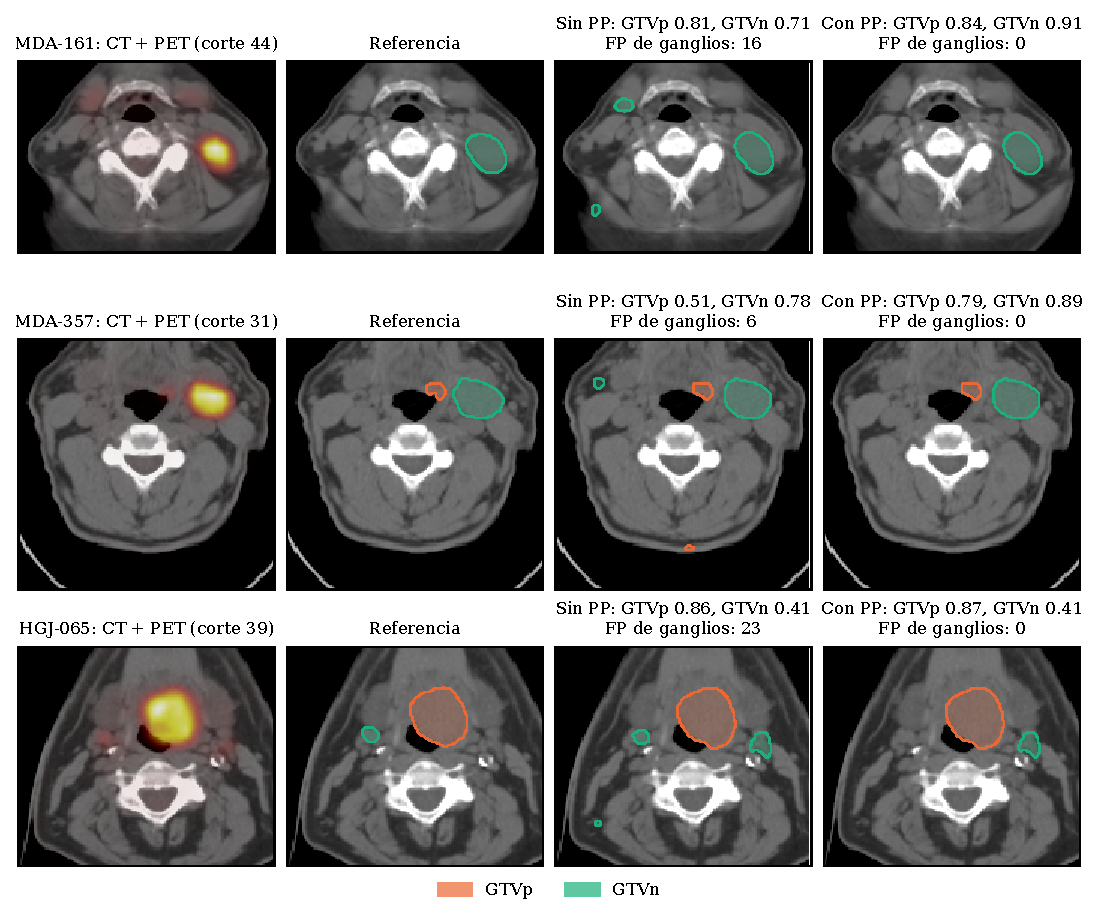
\includegraphics[width=0.86\textwidth]{figuras/postproceso.pdf}
\caption{Predicción de MambaLite3D en tres casos del conjunto de prueba, sin y con postprocesado (PP). Cada fila muestra un corte axial: CT con PET superpuesta, referencia, predicción sin PP y predicción con PP. Los valores de DSC y de falsos positivos (FP) de ganglios corresponden al volumen completo. MDA-161: el PP elimina 16 falsos positivos de ganglios. MDA-357: elimina fragmentos aislados de GTVp. HGJ-065: caso de fallo, en el que el PP elimina un ganglio correcto.}
\label{fig:postproceso}
\end{figure*}

\subsection{Evaluación}

Se usan las métricas de HECKTOR 2025 Tarea 1 y de HECKTOR 2022:
\begin{itemize}
    \item \textbf{GTVp:} DSC medio por paciente. Vale 1 si predicción y referencia están vacías y 0 si solo una lo está.
    \item \textbf{GTVn:} DSC agregado sobre todos los pacientes y F1 de detección. Una lesión se considera detectada si tiene IoU $> 0.3$ con su referencia, con emparejamiento húngaro y conectividad 26.
    \item \textbf{HECKTOR 2022:} DSC agregado de GTVp y GTVn, y su media.
\end{itemize}

El checkpoint se toma al final del entrenamiento (época 250) y no se selecciona por validación. Esta decisión evita elegir el modelo según el conjunto de test.

\section{Resultados}
\label{sec:results}

La Tabla~\ref{tab:test} muestra los resultados en test (69 casos), con y sin postprocesado. La Tabla~\ref{tab:val} muestra la validación final (135 casos), sin postprocesado.

\begin{table}[!t]
\centering
\caption{Resultados en test (69 casos), sin y con postprocesado (PP). La media HECKTOR 2022 usa el DSC agregado de GTVp.}
\label{tab:test}
\footnotesize
\setlength{\tabcolsep}{4pt}
\fitcol{%
\begin{tabular}{l l c c}
\hline
Modelo & Métrica & Sin PP & Con PP \\
\hline
Base (4.0 M) & GTVp DSC & 0.676 & \textbf{0.714} \\
 & GTVn DSCagg & 0.699 & \textbf{0.703} \\
 & GTVn F1agg & 0.345 & \textbf{0.664} \\
 & Media HECKTOR 2022 & 0.719 & \textbf{0.741} \\
\hline
MambaLite3D (15.8 M) & GTVp DSC & 0.679 & \textbf{0.711} \\
 & GTVn DSCagg & 0.704 & \textbf{0.740} \\
 & GTVn F1agg & 0.266 & \textbf{0.703} \\
 & Media HECKTOR 2022 & 0.722 & \textbf{0.760} \\
\hline
\end{tabular}%
}
\end{table}

\begin{table}[!t]
\centering
\caption{Validación final (135 casos), sin postprocesado.}
\label{tab:val}
\footnotesize
\setlength{\tabcolsep}{4pt}
\fitcol{%
\begin{tabular}{l c c c c}
\hline
Modelo & GTVp DSC & GTVn DSCagg & GTVn F1agg & Media 2022 \\
\hline
Base (4.0 M) & 0.619 & 0.686 & 0.308 & 0.690 \\
MambaLite3D (15.8 M) & 0.630 & 0.688 & 0.223 & 0.696 \\
\hline
\end{tabular}%
}
\end{table}

\begin{figure}[!t]
\centering
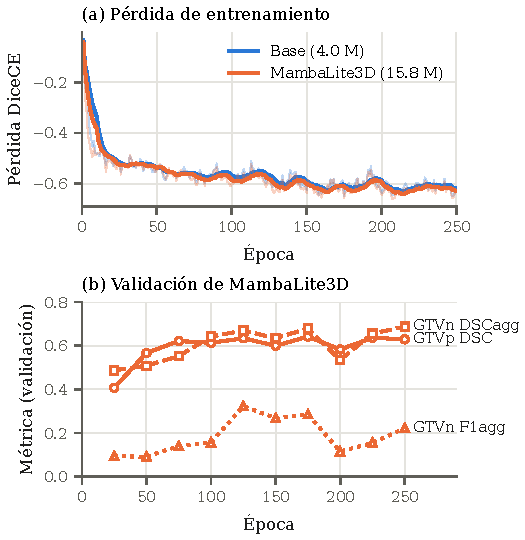
\includegraphics[width=\columnwidth]{figuras/entrenamiento.pdf}
\caption{(a) Pérdida DiceCE por época de ambos modelos; las líneas gruesas son la media móvil de 10 épocas. (b) Métricas de validación de MambaLite3D cada 25 épocas (135 casos, sin postprocesado).}
\label{fig:entrenamiento}
\end{figure}

\begin{figure}[!t]
\centering
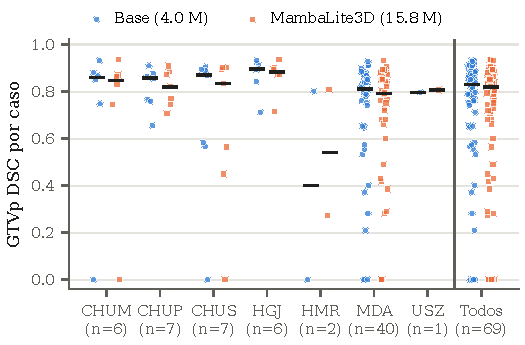
\includegraphics[width=\columnwidth]{figuras/dsc_por_centro.pdf}
\caption{DSC de GTVp por paciente en el conjunto de prueba, con postprocesado, agrupado por centro. Cada punto es un paciente y la raya negra marca la mediana.}
\label{fig:dsc_centro}
\end{figure}

Las curvas de pérdida de ambos modelos son casi coincidentes (Fig.~\ref{fig:entrenamiento}a). Durante el entrenamiento de MambaLite3D, la validación sin postprocesado (135 casos) mejora de forma irregular (Fig.~\ref{fig:entrenamiento}b): el DSC de GTVp pasa de 0.408 (época 25) a 0.642 (época 175), con un valle en la época 200 (0.583), y el DSC agregado de GTVn pasa de 0.487 a 0.688 en la época 250. El F1 de GTVn oscila entre 0.09 y 0.32 y termina en 0.223. La oscilación indica que el resultado depende de la época de corte, lo que refuerza la decisión de usar el checkpoint final.

La Fig.~\ref{fig:postproceso} muestra el efecto del postprocesado en tres casos de prueba. En MDA-161 elimina los 16 falsos positivos de ganglios, y el DSC de GTVn del caso pasa de 0.71 a 0.91. En MDA-357 elimina fragmentos aislados de GTVp, y su DSC pasa de 0.51 a 0.79. HGJ-065 muestra el riesgo de los umbrales: el postprocesado elimina los 23 falsos positivos, pero también uno de los dos ganglios detectados correctamente.

La Fig.~\ref{fig:dsc_centro} muestra el DSC de GTVp por paciente en el conjunto de prueba. La mediana global es de 0.829 en la base y de 0.820 en MambaLite3D, superior a la media (0.714 y 0.711), porque la distribución presenta una cola de fallos completos: 6 casos con DSC nulo en la base y 5 en MambaLite3D, cinco de ellos comunes a ambos modelos (CHUM-038, CHUS-010, MDA-270, MDA-319 y MDA-345). En dos de esos casos por modelo, la referencia no contiene GTVp y el modelo predice una lesión, lo que la métrica puntúa con 0. Los centros HMR y USZ aportan solo 2 y 1 casos de prueba, por lo que sus medianas no son representativas.

\begin{table}[!t]
\centering
\caption{Coste computacional en una NVIDIA GeForce RTX 3050 portátil de 4 GB, según la implementación de Mamba (PyTorch puro o kernels CUDA de \texttt{mamba\_ssm}). Los GFLOPs corresponden a un parche de $32{\times}128{\times}128$; la VRAM de entrenamiento es el pico asignado por iteración (lote de 2 parches, AMP) y la de inferencia, el pico en una ROI de $104{\times}288{\times}448$ vóxeles. La columna Base con \texttt{mamba\_ssm} se midió sin entrenar el modelo completo; $^\dagger$estimado como 62\,500 iteraciones por el tiempo por iteración.}
\label{tab:eficiencia}
\footnotesize
\setlength{\tabcolsep}{4pt}
\fitcol{%
\begin{tabular}{l c c c}
\hline
 & Base & Base & MambaLite3D \\
 & PyTorch & \texttt{mamba\_ssm} & \texttt{mamba\_ssm} \\
\hline
Parámetros (M) & 4.05 & 4.05 & 15.80 \\
GFLOPs por parche & 24.9 & 24.9 & 79.5 \\
VRAM en entrenamiento (GB) & 0.86 & 0.78 & 1.32 \\
Tiempo por iteración (s) & 0.37 & 0.26 & 0.34 \\
Entrenamiento, 250 épocas (h) & 6.5 & 4.5$^\dagger$ & 5.9 \\
VRAM en inferencia (GB) & 0.98 & 0.98 & 1.39 \\
Inferencia por caso (s) & 7.0 & 3.7 & 5.6 \\
\hline
\end{tabular}%
}
\end{table}

\begin{table}[!t]
\centering
\caption{Comparación con trabajos previos en PET/CT de cabeza y cuello. Los valores son los reportados por cada artículo y no son directamente comparables: difieren la edición del desafío, la partición y la métrica.}
\label{tab:sota}
\footnotesize
\setlength{\tabcolsep}{4pt}
\fitcol{%
\begin{tabular}{l l c}
\hline
Método & Evaluación & DSC \\
\hline
nnU-Net + norm. PET \cite{REN2021} & HECKTOR 2021 & 0.779 \\
ISA-Net \cite{isa_net2023} & HECKTOR 2021 & 0.808 \\
SwinCross \cite{Li_2023} & HECKTOR 2021 & 0.769 \\
V-Net 3D \cite{DOUGLAS2025110309} & VC, 10 pliegues & 0.764 \\
UNETR 2.5D \cite{SegmentationHeadNeckDualPETCT2025} & HECKTOR 2022 & 0.818 \\
Swin UNETR \cite{Chu2023114} & HECKTOR 2022, prueba & 0.656 \\
Fusión ponderada \cite{MAHDI2024} & --- & 0.649 \\
\hline
MambaLite3D, GTVp & HECKTOR 2025, interna & 0.711 \\
MambaLite3D, GTVn (agregado) & HECKTOR 2025, interna & 0.740 \\
\hline
\end{tabular}%
}
\end{table}

La Tabla~\ref{tab:eficiencia} resume el coste computacional. La base se entrenó con la implementación en PyTorch puro del barrido selectivo y MambaLite3D con los kernels CUDA de \texttt{mamba\_ssm}; ambas implementaciones son numéricamente equivalentes, ya que, con los mismos pesos, la salida de una capa Mamba difiere en menos de $2\times10^{-7}$ en precisión simple. Para comparar los dos modelos con la misma implementación, medimos además la base con \texttt{mamba\_ssm}. Con este procedimiento, el tiempo por iteración y la memoria de entrenamiento difieren como máximo un 6\,\% de los registrados durante los entrenamientos completos. Con los kernels CUDA, la base reduce su tiempo por iteración de 0.37 a 0.26 s y su inferencia de 7.0 a 3.7 s por caso. Con la misma implementación, MambaLite3D tiene 3.9 veces más parámetros y 3.2 veces más operaciones por parche que la base, pero solo requiere 1.3 veces más tiempo por iteración, 1.7 veces más VRAM de entrenamiento y 1.5 veces más tiempo de inferencia. El pico de VRAM de todo el entrenamiento, incluida la validación periódica, no supera 1.9 GB en ningún modelo, menos de la mitad de la memoria de la GPU empleada.

La Tabla~\ref{tab:sota} sitúa MambaLite3D junto a los resultados reportados por trabajos previos. La comparación es solo orientativa: HECKTOR 2021 evalúa únicamente el tumor primario, mientras que HECKTOR 2022 y 2025 incluyen los ganglios, y nuestros resultados proceden de una partición interna de HECKTOR 2025 y no del conjunto de prueba oficial del desafío. Con esas salvedades, el DSC de GTVp de MambaLite3D (0.711) se sitúa por debajo de los métodos evaluados en HECKTOR 2021 y 2022, salvo Swin UNETR \cite{Chu2023114} y la fusión ponderada \cite{MAHDI2024}.

\section{Discusión}
\label{sec:discusion}

Sin postprocesado, MambaLite3D y la base quedan prácticamente empatados en test (media HECKTOR 2022 de 0.722 frente a 0.719). La base es mejor en F1 de GTVn (0.345 frente a 0.266). Con los datos disponibles no podemos explicar esta diferencia; una hipótesis, que no hemos comprobado, es que el modelo más grande genera más falsos positivos de ganglios antes de filtrar.

El postprocesado mejora mucho el F1 de GTVn en ambos modelos (de 0.27–0.35 a 0.66–0.70). Como las reglas se ajustaron solo en validación, esta mejora no proviene de haber optimizado sobre el test. Con postprocesado, MambaLite3D supera a la base en la media HECKTOR 2022 (0.760 frente a 0.741) y en el DSC agregado de GTVn (0.740 frente a 0.703). En el DSC de GTVp los dos modelos son equivalentes (0.711 frente a 0.714).

Las limitaciones son las siguientes. El test tiene solo 69 casos y la diferencia entre modelos es de unos 0.02 puntos, por lo que puede ser ruido. Todavía no hay una prueba pareada por paciente (bootstrap o Wilcoxon), y se planea hacerla con la herramienta de comparación del proyecto. La comparación entre la base y MambaLite3D solo varía el ancho de los canales, así que no mide el aporte de Mamba frente a una U-Net convolucional. Cada modelo se entrenó con una sola semilla. Las ablaciones (sin Mamba, con el mismo orden de barrido en todos los grupos y sin CGA3D) aún no se han ejecutado, así que no podemos atribuir la diferencia a cada módulo. Las métricas se calcularon con una implementación propia; conviene contrastarlas con el código oficial del challenge antes de compararlas con el leaderboard.

\section{Conclusiones}
\label{sec:conclusiones}

Presentamos MambaLite3D, una U-Net 3D bimodal con Mamba solo en sus niveles más profundos y módulos de mezcla multidireccional, atención local-global y atención cruzada en los skips. Entrenado con un protocolo estratificado por centro en HECKTOR 2025, alcanza en test con postprocesado un DSC de GTVp de 0.711, un DSC agregado de GTVn de 0.740 y un F1 de detección de GTVn de 0.703. Frente a la variante base de la misma arquitectura, la mejora es pequeña y requiere confirmación estadística. Los trabajos siguientes son las ablaciones, la prueba pareada por paciente y varias semillas para estimar la variabilidad.

\section*{Agradecimientos}
% Pendiente: agregar agradecimientos.

\bibliographystyle{IEEEtran}
\bibliography{references}

\end{document}
